\documentclass{article}
\usepackage[finnish]{babel}
\usepackage[utf8]{inputenc}
\usepackage{graphicx}
\author{Jaakko Hannikainen}

\title{Tietorakenteiden ja algoritmien harjoitustyö - Viikkoraportti 2}
\begin{document}
\maketitle

\section{Mitä opin tällä viikolla}
\begin{itemize}
    \item gnuplotin syntaksia
    \item maken syntaksia mystisiltä osilta
\end{itemize}

\section{Mitä jäi epäselväksi}
\begin{itemize}
    \item gnuplotin syntaksi
    \item ohjelman kehityssuunta
\end{itemize}

\section{Miten ohjelma on edistynyt?}
\begin{itemize}
    \item dynaminen luonti
    \item parempi line-of-sight
    \item kolme sokkelonluontialgoritmia; tyhjä, prim ja life
    \item testit kattavat kaikki datarakenteiden rivit
    \item paljon siistimpi koodirakenne kuin edellisessä palautuksessa
    \item 3d-grafiikat
    \item 3d-avaruudessa liikkuminen
\end{itemize}

\section{Mitä teen seuraavaksi?}
\begin{itemize}
    \item vihollisia, esineitä yms. muuta pelillistämistä?
    \item seinien poistaminen ja lisääminen, inventory
    \item 3d-maailma
    \item lisää generaattoreita
    \item optimointia
\end{itemize}

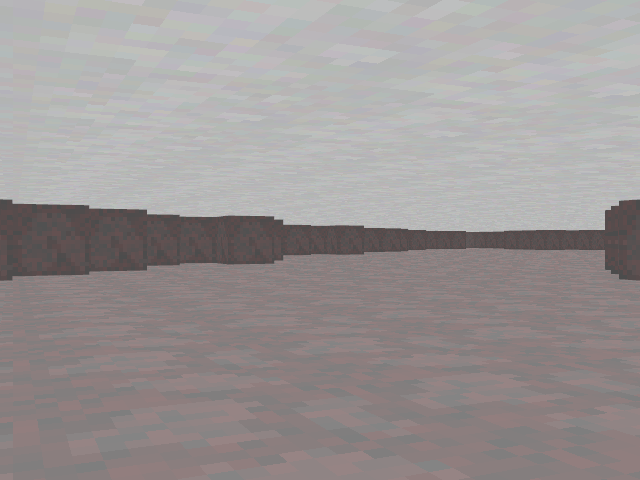
\includegraphics[scale=0.5]{vk2-screen}

\end{document}
